\documentclass[conference]{IEEEtran}
\usepackage{cite,amsmath,amssymb,graphicx,booktabs,multirow,xcolor,url,algorithm,algpseudocode}
\usepackage{tikz}
\usetikzlibrary{arrows.meta,positioning,fit}
\usepackage[hidelinks]{hyperref}
% \tbd marks numbers that are filled in from results/ after the GPU run. Remove before submission.
\newcommand{\tbd}[1]{\textcolor{red}{[#1]}}
\graphicspath{{figures/}}

\begin{document}
\title{TrialMatch-LLM: Evidence-Grounded Criterion-Level Clinical-Trial Screening with a Fine-Tuned Small Decoder, Explicit KV Caching, Tiled Attention and Speculative Decoding}

\author{\IEEEauthorblockN{\tbd{Your Name}}
\IEEEauthorblockA{\tbd{Roll number}, \tbd{Department}, \tbd{University}\\ \tbd{email}}}

\maketitle

\begin{abstract}
We build and evaluate a complete, locally executable Transformer system that decides how individual inclusion and exclusion criteria of a clinical trial apply to a patient and cites the supporting patient sentences. Using only the TrialGPT Criterion Annotations dataset and a fixed patient-grouped 37/8/8 split, we fine-tune Qwen2.5-1.5B-Instruct with LoRA to emit a JSON object containing evidence sentence IDs followed by one of four expert label categories, including \emph{not enough information} and \emph{not applicable}. On the held-out test patients, fine-tuning changes accuracy from \tbd{x} to \tbd{y} and macro-F1 from \tbd{x} to \tbd{y}, and evidence micro-F1 from \tbd{x} to \tbd{y}. We additionally implement, from scratch, a Qwen2 forward pass with an explicit key/value cache (token-identical to an uncached reference at all tested lengths, \tbd{N}$\times$ faster decoding at 1024 input tokens), a tiled online-softmax attention kernel (max.\ error \tbd{e} vs.\ fp64), and greedy speculative decoding with a 0.5B draft (token-identical outputs, acceptance \tbd{a}\%, speed-up \tbd{s}$\times$). All components are exposed in a browser application that screens unseen notes and exports a provenance-tagged report.
\end{abstract}

\begin{IEEEkeywords}
clinical trial matching, large language models, LoRA, KV cache, FlashAttention, speculative decoding, evidence extraction
\end{IEEEkeywords}

%=====================================================================
\section{Introduction}
Recruitment is a major bottleneck of clinical trials, and checking a patient against dozens of free-text eligibility criteria is laborious. TrialGPT~\cite{jin2024trialgpt} showed that large proprietary models can predict criterion-level eligibility and cite evidence. Our goal is a system that (i) runs entirely on free hardware with open weights, (ii) preserves the full label space, including insufficient-information and not-applicable outcomes rather than forcing a yes/no decision, (iii) grounds every decision in patient sentence IDs, and (iv) makes the inference mechanisms that dominate cost (KV caching, attention, decoding) explicit and verified.

\textbf{Problem statement.} Given a patient note split into numbered sentences $S=\{s_0,\dots,s_{n-1}\}$, a criterion type $t\in\{\text{inclusion},\text{exclusion}\}$ and criterion text $c$, predict a label $y\in\mathcal{Y}_t$ and an evidence set $E\subseteq\{0,\dots,n-1\}$, where $\mathcal{Y}_{\text{inc}}=\{$included, not included, not enough information, not applicable$\}$ and $\mathcal{Y}_{\text{exc}}=\{$excluded, not excluded, not enough information, not applicable$\}$.

\textbf{Contributions.} (1) A leakage-controlled fine-tuning and evaluation pipeline with the mandated split; (2) a from-scratch cache-aware Qwen2 decoder with prefix caching; (3) a tiled online-softmax attention kernel; (4) a greedy speculative decoder with explicit cache rollback; (5) a browser application with live benchmarks; (6) an honest analysis including failures and slow-downs.

%=====================================================================
\section{Related Work}
\textbf{Patient--trial matching.} The patients in our data originate from the SIGIR 2016 test collection~\cite{koopman2016test}. TrialGPT~\cite{jin2024trialgpt} prompts GPT-4 to produce criterion-level labels, explanations and evidence sentences, then aggregates them into trial rankings. It relies on a proprietary API; we instead study what a 1.5B open model can learn from the expert annotations, and we never use the GPT-4 predictions stored in the dataset.

\textbf{Transformers and efficient adaptation.} We build on the decoder-only Transformer~\cite{vaswani2017attention} with rotary position embeddings~\cite{su2024roformer} and grouped-query attention (GQA)~\cite{ainslie2023gqa}, as used by Qwen2.5~\cite{qwen2025qwen25} and Llama~3~\cite{dubey2024llama3}. LoRA~\cite{hu2022lora} trains low-rank updates $\Delta W=\tfrac{\alpha}{r}BA$ while freezing $W$; QLoRA~\cite{dettmers2023qlora} additionally quantises $W$ to 4-bit NF4. Full fine-tuning of a 1.5B model needs about 4$\times$ the weight memory for Adam states and would over-fit 602 examples; LoRA trains $<$\tbd{1.2}\% of the parameters. QLoRA reduces frozen-weight memory about 4$\times$ at the cost of de-quantisation overhead and quantisation error; on a 16\,GB T4 the 1.5B model fits without it (\S\ref{sec:decisions}).

\textbf{Efficient inference.} Pope et al.~\cite{pope2023efficiently} analyse KV-cache memory and why autoregressive decoding is memory-bandwidth bound; PagedAttention~\cite{kwon2023pagedattention} manages cache memory in blocks. FlashAttention~\cite{dao2022flashattention} computes exact attention in SRAM tiles using the online softmax normaliser of Milakov and Gimelshein~\cite{milakov2018online}, avoiding the $O(T^2)$ score matrix. Speculative decoding~\cite{leviathan2023fast,chen2023accelerating} lets a cheap draft model propose $k$ tokens that the target verifies in one forward pass; under greedy acceptance the output is provably identical to target-only greedy decoding. Limitations: speed-ups require high acceptance and a draft that is much cheaper than the target, which is not guaranteed for short structured outputs (\S\ref{sec:spec}).

%=====================================================================
\section{Materials and Methods}
\subsection{Dataset, split and leakage control}
The dataset has 1{,}015 criterion annotations for 53 patients and 103 trials. We drop \texttt{gpt4\_explanation}, \texttt{gpt4\_sentences}, \texttt{gpt4\_eligibility}, \texttt{explanation\_correctness} and the dataset's own \texttt{training} flag immediately after loading (an assertion guards against regressions). Following the protocol, unique patient IDs are sorted, shuffled with \texttt{numpy.random.default\_rng(42)}, and assigned 37/8/8 to train/validation/test. One training annotation with empty criterion text was removed after splitting (recorded in the manifest), giving 602/206/206 annotations. Table~\ref{tab:data} shows the label distribution: it is highly imbalanced (\emph{not excluded} dominates exclusion criteria) and the test split contains \emph{no} \emph{excluded} example, so that class's test recall is undefined; we report it on validation instead. 60\% of annotations have no gold evidence sentence. The manifest (\texttt{splits/manifest.json}) lists patient IDs and per-patient counts, and unit tests verify the protocol and disjointness.

\begin{table}[t]\centering\caption{Label distribution per split (annotations).}\label{tab:data}
\begin{tabular}{llrrr}\toprule
Type & Label & Train & Val & Test\\\midrule
\multirow{4}{*}{Inclusion} & included & 88 & 35 & 27\\
 & not included & 13 & 3 & 7\\
 & not enough information & 109 & 27 & 38\\
 & not applicable & 5 & 1 & 3\\\midrule
\multirow{4}{*}{Exclusion} & excluded & 8 & 2 & 0\\
 & not excluded & 291 & 101 & 91\\
 & not enough information & 65 & 26 & 28\\
 & not applicable & 23 & 11 & 12\\\midrule
 & Patients / annotations & 37/602 & 8/206 & 8/206\\\bottomrule
\end{tabular}\end{table}

\subsection{Input/output format and truncation}
The prompt (Qwen chat format) contains a system instruction, the patient note as \texttt{[id] sentence} lines using the dataset's original sentence IDs, the criterion type, the criterion text, and the allowed labels for that type. The target is \texttt{\{"evidence\_ids":[\dots],"label":"\dots"\}<|im\_end|>}. Placing evidence \emph{before} the label conditions the decision on the cited sentences. The prompt is tokenised as a \emph{patient prefix} and a \emph{criterion suffix}; the same function is used in training, evaluation and the application, which makes prefix-KV reuse across criteria exact. If a prompt exceeded 1{,}800 tokens, patient sentences would be dropped from the end and logged with a flag if gold evidence was lost; with the Qwen tokenizer the longest prompt is 610 tokens (mean \tbd{326}), so \textbf{no example was truncated} (audit in the manifest). Explanations are generated deterministically from the predicted label and the quoted cited sentences; this guarantees that an explanation cannot introduce facts absent from the record and avoids training on GPT-4 explanations. Outputs are parsed strictly as JSON; a fallback searches for an allowed label string; otherwise the prediction is \emph{invalid} and counted as wrong.

\subsection{Model selection}
Table~\ref{tab:models} compares the candidates. We select Qwen2.5-1.5B-Instruct: Apache-2.0 licence (no gating), GQA with only 2 KV heads (28\,KB of fp16 KV cache per token, 6$\times$ less than multi-head attention), a 151{,}936-token vocabulary shared with the 0.5B sibling that serves as a speculative draft, and fp32 weights (6.2\,GB) that fit a free 16\,GB T4 for LoRA training without quantisation. Llama-3.2-1B has a more restrictive community licence and a gated download, and Llama-3.2-3B leaves little memory for training on a T4.

\begin{table}[t]\centering\caption{Open-weight decoder candidates.}\label{tab:models}\setlength{\tabcolsep}{3pt}
\begin{tabular}{lccc}\toprule
 & Qwen2.5-1.5B-I & Qwen2.5-0.5B-I & Llama-3.2-1B-I\\\midrule
Params & 1.54B & 0.49B & 1.24B\\
Layers / hidden & 28 / 1536 & 24 / 896 & 16 / 2048\\
Q / KV heads & 12 / 2 & 14 / 2 & 32 / 8\\
Context & 32{,}768 & 32{,}768 & 131{,}072\\
Vocabulary & 151{,}936 & 151{,}936 & 128{,}256\\
Licence & Apache-2.0 & Apache-2.0 & Llama 3.2 Comm.\\
fp16 weights & 3.1\,GB & 1.0\,GB & 2.5\,GB\\
KV / token (fp16) & 28\,KB & 12\,KB & 32\,KB\\
Role & target & draft & rejected\\\bottomrule
\end{tabular}\end{table}

\subsection{Fine-tuning}
Objective: token-level cross-entropy on the answer tokens only (prompt tokens masked with $-100$). LoRA ($r{=}16$, $\alpha{=}32$, dropout 0.05) is applied to all attention and MLP projections (\tbd{18.5M} trainable parameters, \tbd{1.2}\%). AdamW, learning rate $2\times10^{-4}$, cosine schedule with 5\% warm-up, effective batch 16 (4$\times$4 accumulation), 3 epochs, fp32 base weights with fp16 autocast, seed 42, on one Kaggle T4 (\tbd{time}, peak \tbd{GB}). A checkpoint is saved every epoch; the final model is the checkpoint with the best \emph{validation} macro-F1 (tie-break: evidence micro-F1). The test split is only accessible with an explicit \texttt{--final\_test} flag and was evaluated once.

\subsection{System architecture}
Fig.~\ref{fig:arch} shows the pipeline. The LoRA adapter is merged into the base weights ($W\leftarrow W+\tfrac{\alpha}{r}BA$) so that all inference code sees a dense model.

\begin{figure}[t]\centering
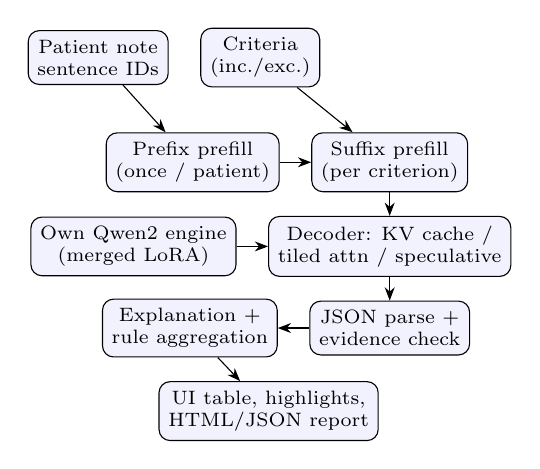
\begin{tikzpicture}[node distance=3mm and 4mm, every node/.style={font=\scriptsize}, box/.style={draw,rounded corners,align=center,minimum height=6mm,fill=blue!5}, >=Stealth]
\node[box] (note) {Patient note\\sentence IDs};
\node[box,right=of note] (crit) {Criteria\\(inc./exc.)};
\node[box,below=6mm of note,xshift=12mm] (pre) {Prefix prefill\\(once / patient)};
\node[box,right=of pre] (suf) {Suffix prefill\\(per criterion)};
\node[box,below=of suf] (dec) {Decoder: KV cache /\\tiled attn / speculative};
\node[box,left=of dec] (eng) {Own Qwen2 engine\\(merged LoRA)};
\node[box,below=of dec] (parse) {JSON parse +\\evidence check};
\node[box,left=of parse] (agg) {Explanation +\\rule aggregation};
\node[box,below=of agg,xshift=10mm] (out) {UI table, highlights,\\HTML/JSON report};
\draw[->] (note) -- (pre); \draw[->] (crit) -- (suf); \draw[->] (pre) -- (suf); \draw[->] (suf) -- (dec);
\draw[->] (eng) -- (dec); \draw[->] (dec) -- (parse); \draw[->] (parse) -- (agg); \draw[->] (agg) -- (out);
\end{tikzpicture}
\caption{TrialMatch-LLM inference workflow. The patient prefix KV cache is computed once and reused for every criterion.}\label{fig:arch}
\end{figure}

\subsection{Cache-aware decoding (Task 3)}
Our engine re-implements the Qwen2 forward pass (embedding, RMSNorm, RoPE, GQA, SwiGLU, tied LM head) using the model's weights; its logits match Hugging Face within $10^{-4}$ (fp32 unit test). The cache stores, per layer, $K,V\in\mathbb{R}^{B\times h_{kv}\times C\times d}$ with a valid length $L$. \emph{Positional handling:} a token at absolute position $p$ is rotated by $p\,\theta_i$ \emph{before} its key is written, so cached keys are never re-rotated; a step feeding token $x_L$ only needs position $L$. \emph{Masking:} prefill uses a causal mask; when $T_q$ new queries attend to $L+T_q$ keys the mask is bottom-right aligned (query $i$ sees keys $j\le L+i$). For single-token decoding all cached keys are visible and no mask is needed. Note that PyTorch's \texttt{is\_causal=True} is top-left aligned and would be wrong for $T_q<T_k$, so we pass explicit masks. \emph{Growth:} buffers are pre-allocated and doubled when full (amortised $O(1)$ per token); memory is $2\,N_{\text{layers}}\,h_{kv}\,d\,b$ bytes per token ($b$ bytes per element). \emph{Rollback:} cropping only resets $L$. The reference path recomputes the whole sequence every step. We also include a loop that passes an explicitly constructed \texttt{DynamicCache}, positions and \texttt{cache\_position} to the HF model, to separate the effect of our engine from the effect of caching.

\subsection{Tiled online-softmax attention (Task 4)}
Algorithm~\ref{alg:tiled} processes query blocks of size $B_q$ and streams key/value blocks of size $B_k$, keeping a running row maximum $m$, normaliser $\ell$ and un-normalised output $O$. Blocks entirely in the causal future are skipped, and only blocks that straddle the diagonal are masked. Extra memory is $O(B_qB_k)$ instead of $O(T^2)$.

\begin{algorithm}[t]\caption{Tiled attention with online softmax}\label{alg:tiled}\small
\begin{algorithmic}[1]
\For{each query block $Q_i$}
 \State $m\gets-\infty$, $\ell\gets 0$, $O\gets 0$
 \For{each key block $(K_j,V_j)$ not entirely in the future}
  \State $S\gets Q_iK_j^\top/\sqrt d$; mask future positions with $-\infty$
  \State $m'\gets\max(m,\operatorname{rowmax}S)$; $\alpha\gets e^{m-m'}$; $P\gets e^{S-m'}$
  \State $\ell\gets\alpha\ell+\operatorname{rowsum}P$; $O\gets\alpha O+PV_j$; $m\gets m'$
 \EndFor
 \State output block $i$: $O/\ell$
\EndFor
\end{algorithmic}\end{algorithm}

\subsection{Greedy speculative decoding (Task 5)}\label{sec:specmethod}
Invariant: with committed sequence $x_{1:n}$, the target cache holds $x_{1:n-1}$, and the draft cache holds a prefix of it. Each round (i) the draft greedily proposes $d_1..d_k$, feeding any committed tokens it has not cached; (ii) the target runs \emph{one} forward pass over $[x_n,d_1..d_k]$ and returns $t_1..t_{k+1}$; (iii) the longest prefix with $d_i=t_i$ ($a$ tokens) is accepted and $t_{a+1}$ is appended (the correction on rejection, or a bonus token if $a{=}k$); (iv) both caches are cropped to $n+a$ entries, discarding the K/V of rejected tokens. Each round therefore emits between 1 and $k{+}1$ tokens that are identical to target-only greedy decoding. The draft is Qwen2.5-0.5B-Instruct (identical tokenizer, verified programmatically); we compare it to a draft fine-tuned with LoRA on the same training split.

\subsection{Application}
A Gradio application (Fig.~\tbd{screenshot}) is started with \texttt{start.bat}/\texttt{start.sh}. It accepts unseen free-text notes (automatically sentence-split) and criteria, validates inputs (empty or short notes, too many or too long criteria, context overflow warnings), lets the user choose the inference mode, and shows per-criterion labels, cited IDs, evidence text, explanations, and missing-information flags, with the cited sentences highlighted. The preliminary patient--trial outcome is an explicit rule: \emph{likely ineligible} if any inclusion criterion is \emph{not included} or any exclusion criterion is \emph{excluded}; otherwise \emph{needs review} if any criterion has insufficient information; otherwise \emph{likely eligible}. It is not a ground-truth label. Reports are exported as HTML and JSON with provenance (model, adapter, decoding mode, device, input hash, timestamp). A benchmark tab runs all decoding paths live on the user's input.

%=====================================================================
\section{Experimental Setup and Metrics}
\textbf{Hardware.} Training and GPU benchmarks: Kaggle, 1$\times$ NVIDIA T4 (16\,GB, no bf16), \tbd{torch/transformers versions}. Application: Intel Core i5-10210U laptop CPU, 24\,GB RAM, fp32.
\textbf{Decoding.} Greedy, \texttt{max\_new\_tokens}=64, batch 8 with left padding for metric evaluation; identical prompts and rows before and after fine-tuning.
\textbf{Classification.} Accuracy, macro-F1 over the gold classes present, per-class P/R/F1 and confusion matrices for inclusion, exclusion, and overall (8 type-specific classes).
\textbf{Evidence.} Micro P/R/F1 sums TP/FP/FN over rows; macro averages row-level scores. Empty-set conventions: gold $=\emptyset$ and prediction $=\emptyset$ scores 1; exactly one empty scores 0. Because 60\% of rows have empty gold evidence, we also report metrics restricted to rows with non-empty gold evidence (no convention needed) and the counts of the four empty/non-empty patterns.
\textbf{Timing.} One warm-up run, then 3 repeats with \texttt{torch.cuda.synchronize()} around each phase; median reported. Peak memory from \texttt{torch.cuda.max\_memory\_allocated}. EOS is disabled for fixed-length KV benchmarks.

%=====================================================================
\section{Results and Discussion}
\subsection{Fine-tuning and before/after comparison}
Fig.~\ref{fig:curves} shows the training curves (\tbd{interpretation: e.g. validation loss minimum at epoch k}). Table~\ref{tab:main} compares the base and fine-tuned model on identical validation and test rows. \tbd{Discussion: the base model mostly outputs X, over-predicts Y, invalid rate Z; after fine-tuning ...}

\begin{figure}[t]\centering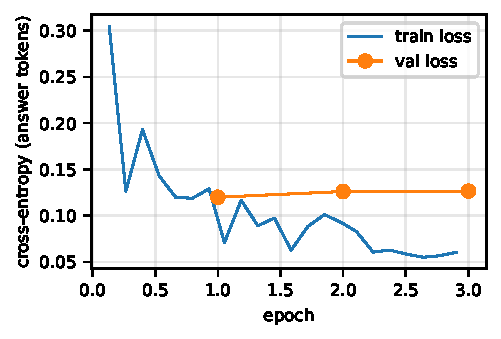
\includegraphics[width=\columnwidth]{training_curves}
\caption{LoRA training and validation loss.}\label{fig:curves}\end{figure}

\begin{table*}[t]\centering\caption{Criterion classification and evidence retrieval (greedy, same rows). Ev.\ = evidence; $>0$ = rows with non-empty gold evidence.}\label{tab:main}
\begin{tabular}{llcccccccc}\toprule
Split & Model & Acc. & Macro-F1 & Inc.\ mF1 & Exc.\ mF1 & Ev.\ micro-F1 & Ev.\ macro-F1 & Ev.\ micro-F1 ($>0$) & Strict JSON\\\midrule
% split & model & acc & macroF1 & inc-mF1 & exc-mF1 & ev-microF1 & ev-macroF1 & ev-microF1(gold>0) & parse
val & base & 0.141 & 0.103 & 0.198 & 0.007 & 0.188 & 0.464 & 0.311 & 1.00 \\
val & ft-best & 0.694 & 0.353 & 0.328 & 0.378 & 0.530 & 0.703 & 0.631 & 1.00 \\
test & base & 0.228 & 0.192 & 0.336 & 0.000 & 0.236 & 0.608 & 0.403 & 1.00 \\
test & ft-best & 0.694 & 0.386 & 0.379 & 0.395 & 0.546 & 0.790 & 0.651 & 1.00 \\

\bottomrule\end{tabular}\end{table*}

\subsection{Detailed classification and evidence analysis}
Fig.~\ref{fig:cm} shows the test confusion matrices. \tbd{Per-class discussion: NEI vs. definite labels, rare classes not included/excluded, not applicable.} \tbd{Evidence: precision vs. recall, empty-pattern counts.}

\begin{figure}[t]\centering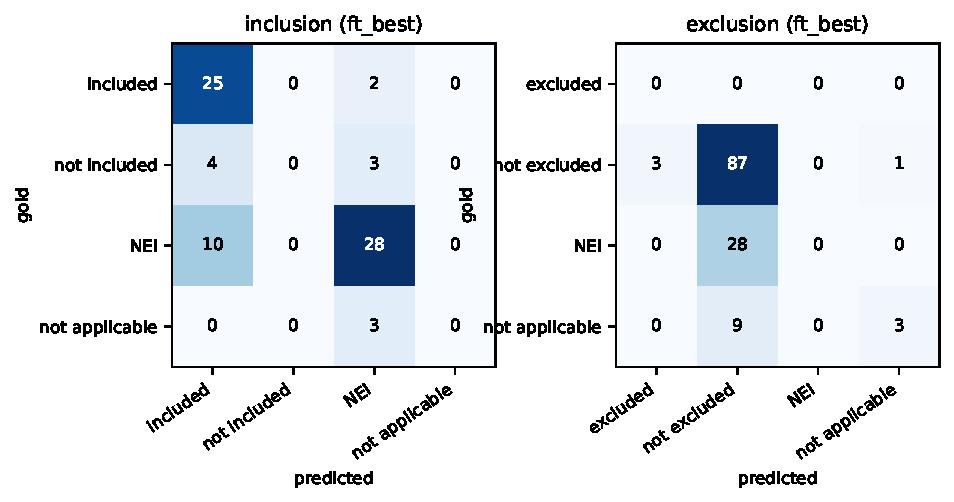
\includegraphics[width=\columnwidth]{confusion_test_ft_best}
\caption{Test confusion matrices of the fine-tuned model (NEI = not enough information).}\label{fig:cm}\end{figure}

\subsection{Error analysis}
Using the automatic taxonomy in \texttt{scripts/error\_analysis.py} (E1--E9), we analyse at least eight distinct test errors: \tbd{(1) unsupported certainty: ... (2) missed information ... (3) polarity ... (4) not applicable ... (5) definite label without evidence ... (6) spurious citation ... (7) correct label, wrong evidence ... (8) contradictory: right evidence, wrong label ...}. In line with the protocol, absence of evidence is never treated as proof: \tbd{how often the model predicts a definite label with no cited sentence}.

\subsection{KV cache}
Table~\tbd{kv} and Fig.~\ref{fig:kv}: all paths produce identical greedy tokens for input lengths 128/512/1024 and output lengths 32/128/256 \tbd{(or: first mismatch at step s, top-2 logit margin m)}. Cached decoding throughput is roughly constant in sequence length while uncached cost grows with $T$, yielding \tbd{N}$\times$ at 1024+256 tokens. The cache costs \tbd{MB} at 1280 tokens, consistent with 28\,KB/token. \emph{Numerical differences:} cached and uncached paths compute the same mathematical function, but in fp16 the reduction order differs (matrix-vector vs.\ matrix-matrix kernels), so logits differ by \tbd{measured magnitude} and argmax flips are possible only at near-ties.

\begin{figure}[t]\centering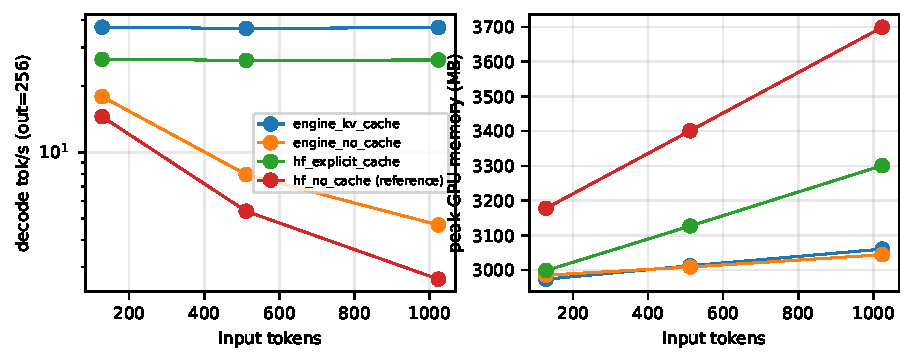
\includegraphics[width=\columnwidth]{kv_cache_bench}
\caption{Decode throughput and peak memory, cached vs.\ uncached.}\label{fig:kv}\end{figure}

\subsection{Tiled attention}
Our tiled kernel matches the fp64 reference with maximum error \tbd{e} (fp32) and \tbd{e} (fp16) over all shapes, masks and block sizes (Fig.~\ref{fig:attn}). It is \tbd{x}$\times$ slower than PyTorch SDPA because each tile is a separate Python-level kernel launch, intermediate tiles are written to and read back from HBM instead of staying in on-chip SRAM, and the rescaling adds element-wise passes; a fused kernel performs the entire loop inside one CUDA kernel. Its memory advantage over the reference (which materialises $T^2$ scores: 12 heads$\times4096^2\times2$\,B $=$ 384\,MB at $T{=}4096$) is nonetheless visible.

\begin{figure}[t]\centering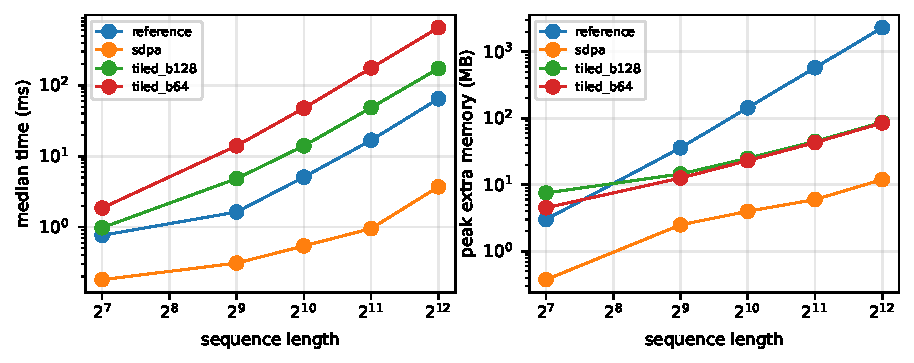
\includegraphics[width=\columnwidth]{attention_bench}
\caption{Attention runtime and extra memory vs.\ sequence length (T4, fp16).}\label{fig:attn}\end{figure}

\subsection{Speculative decoding}\label{sec:spec}
Fig.~\ref{fig:spec}: outputs are token-identical to greedy decoding for every prompt and $k$. \tbd{Acceptance x\%, best k, speed-up or slow-down.} \tbd{Explain: the 0.5B draft costs about 1/3 of the target per token on a T4 at batch 1 because both are launch/latency bound, so the theoretical speed-up $\frac{1-\alpha^{k+1}}{(1-\alpha)(1+k c)}$ with cost ratio $c\approx$ \dots is small; the JSON answers are short (around 20 tokens); a fine-tuned draft raises acceptance from x to y.}

\begin{figure}[t]\centering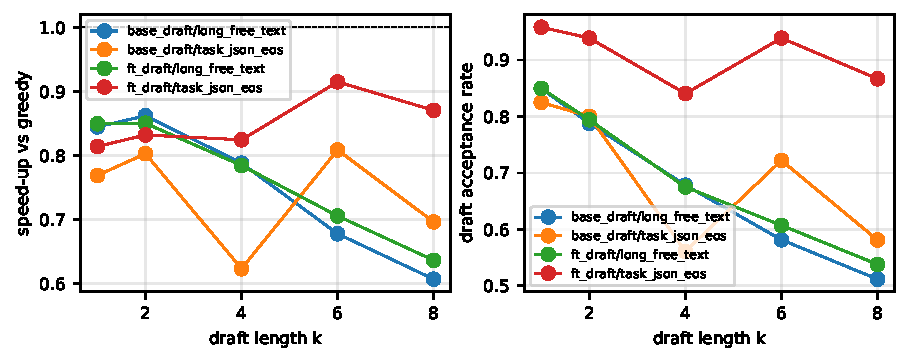
\includegraphics[width=\columnwidth]{speculative_bench}
\caption{Speculative decoding speed-up and acceptance vs.\ draft length $k$.}\label{fig:spec}\end{figure}

\subsection{Design decisions, alternatives and failures}\label{sec:decisions}
\begin{itemize}
\item \textbf{LoRA vs.\ QLoRA vs.\ full FT:} \tbd{...}
\item \textbf{Evidence-first JSON vs.\ label-first:} \tbd{...}
\item \textbf{Template explanations vs.\ generated rationales:} generated rationales would require GPT-4 explanations as training targets (excluded) and can hallucinate; we chose faithful templates.
\item \textbf{Prefix caching} across criteria saves \tbd{x}\% of prefill time in the application.
\item \textbf{Failures observed:} \tbd{e.g., base model produced prose instead of JSON; \texttt{is\_causal} mask misalignment; transformers v5 API changes (\texttt{warmup\_ratio}); fp16 near-tie mismatches.}
\end{itemize}

%=====================================================================
\section{Limitations}
Small data (602 training annotations, 37 patients) and severe class imbalance (8 training \emph{excluded} examples, none in test) make per-class results for rare classes unreliable; 8 test patients give wide confidence intervals. Notes are short, synthetic-style SIGIR topics rather than full EHRs. The 1.5B model has limited medical knowledge. Explanations are faithful but shallow. CPU inference is slow (seconds per criterion). Speculative decoding gains are hardware-dependent. The aggregated outcome is a heuristic, not validated against trial enrolment. The system is an educational prototype and must not be used for clinical decisions.

\section{Conclusion}
\tbd{Summarise the main quantitative findings and lessons.}

\appendices
\section{AI-use statement}
An AI coding assistant (Anthropic Claude) was used to draft code scaffolding, unit tests and parts of this report's text. All code was reviewed, executed and tested by the author (41 unit tests); all numbers come from logged runs in the repository. Design decisions, analysis and verification are the author's own responsibility.

\section{Reproducibility}
Code: \tbd{GitHub URL}. Adapter: \tbd{HF URL}. Split manifest: \texttt{splits/manifest.json}. Logs: \texttt{results/}. Demo video: \tbd{URL}.

\bibliographystyle{IEEEtran}
\bibliography{refs}
\end{document}
